%% LyX 2.0.4 created this file.  For more info, see http://www.lyx.org/.
%% Do not edit unless you really know what you are doing.
\documentclass[english]{article}
\usepackage[T1]{fontenc}
\usepackage[utf8]{luainputenc}
\usepackage{amsmath}
\usepackage{amssymb}
\usepackage{graphicx}
\usepackage{esint}

\makeatletter

%%%%%%%%%%%%%%%%%%%%%%%%%%%%%% LyX specific LaTeX commands.
%% Because html converters don't know tabularnewline
\providecommand{\tabularnewline}{\\}

%%%%%%%%%%%%%%%%%%%%%%%%%%%%%% User specified LaTeX commands.
\usepackage{babel}

\makeatother

\usepackage{babel}
\begin{document}

\title{Weak Lensing Shear Inference:A Hierarchy Bayesian Approach}


\date{02/16/2013}
\maketitle
\begin{abstract}
We present a Hierarchy Bayesian method for shear inference in Weak
Lensing survey. With this method we are able to infer synchronously
cosmic shear at different sky patches as well as the intrinsic shape
distribution. We show that this Hierarchy Bayesian method is more
accurate than the traditional average method and (prove to a large
extent )it is an unbiased estimation of shear.

Key words:gravational lensing-methods;data analysis-methods;bayesian
inference 
\end{abstract}

\section{Introduction}

$\ \ \ \ $Weak Lensing has become one of the most powerful method
in exploring the distribution of matter in the Universe on large scales
(Bartelmann \& Schneider 2001,Al- brecht et al. 2006; Peacock \& Schneider
2006 ).This powerful method has a various astronomical applications.By
detecting the weak lensing shear or magnification effect we are able
to reconstruct the mass properties of galaxy clusters,as well as dark
matter halos(Dahle et al. 2002; Gray et al. 2002; Clowe, Gonzalez
\& Markevitch 2004;Sheldon et al. 2004)

General relativity predicts that the path of light from a distant
galaxy is distorted by the gravitational potential fluctu- ations
along the line of sight. As dark energy slows the growth of dark matter
structures, these in turn affect the appearance of distant galaxies,
distorting them slightly as gravitational fields deflect their light.
This distortion is known as cosmic shear.()

The measurement of cosmic shear is determined by the amount of distortion
caused to foreground galaxies. Due to the isotropy of the Universe
the expect value of the intrinsic complex ellipticity $\epsilon$
of a galaxy is 0. Therefore the complex ellipticity of a stretched
galaxies is an unbiased estimation of cosmic shear(Bartelmann \& Schneider
2001).However, the distortion induced by cosmic shear is typically
on the order of a few percent,which is significantly smaller than
the galaxies's intrinsic shape noise(\textasciitilde{}0.1 level).

Several beysian or likelihood approaches towards shear measurement
like lensfit(L. Miller,T. D. Kitching et al,2007;T.D. Kitching, L.
Miller et al 2008 ) im2shape(Bridle,) im3shape(Joe Zuntz, et al,arxive2013)
have bean make recently.{[}im3shape fitted different models on galaxies
image and used a max-likelihood method to determin the model parameters,and
then obtain the galaxy's ellipticity.{]}{[}lensfit proposed a modelfitting
approach in the galaxy shape measurement and evaluated how shear sensitivity
should be calculated based on posterior distribution of galaxies shape.{]}
However these methods mostly focus on the shape measurement of a single
galaxy.Given an telescope that has perfect measurement on galaxies'
shape their shear estimation method has no difference from traditional
averaging method.

While in this paper what we want to focus is how a hierarchy beysian
approach can infer cosmic shear independently from which way the galaxy
shape is measured with better accuracy than traditional averaging
method.Therefore in the toy model we used,we assume we have perfect
measurement on the galaxy shape.

One of the major problems of a bayesian inference of cosmic shear
is that even though a lot of measurement have bean made ,we still
know little about the intrinsic ellipticity distribution of galaxies
of the whole universe(Leauthaud\&Massey 2007;Joachimi\&Semboloni2012).However
in our Hierarchy Bayesian method we avoid to making up any empirical
model for intrinsic ellipticity distribution.We will show that using
a free form model for intrinsic ellipticity distribution and infer
its parameters together with cosmic shear we can still out perform
the traditional average method.

The graphic model describe the hierarchy bayesian method in detail.
We assume in one sky patch there is a uniform

shear that applies on all the galaxies in that patch,and galaxies
in all patches have the same intrinsic ellipticity distribution.In
this way even if the number of galaxies in one patch is small,if we
have enough sky patches we can still get a good estimation of $\alpha$,which
is the key to have a good estimation of shear $g$ in each patch which
is the quantity we cares about.

\includegraphics[scale=0.5]{yike}

This report is orgnized as following: First we introduce the lensing
formula used in weak lensing region and how we simulated the lensed
ellpticity of galaxies.Then we introduced the likelihood function
$P(\epsilon_{\ell}|g,\alpha)$ which is the probability of having
lensed ellipticity $\epsilon_{\ell}$ given reduced shear $g$ in
each patch and intrinsic ellipticity $\epsilon_{0}$distribution parameter
$\alpha$ .Finally we show some results of the posterior distribution
sampling for two different models we selected for intrinsic shape
distrition function.Finally we estimate the level of possible systematic
bias of this HB inference.


\section{Method}


\subsection{Data Generation}

$\ \ \ \ $The definition of complex ellipticity of a galaxy is 
\begin{equation}
\epsilon=\frac{1-q}{1+q}e^{2i\phi}
\end{equation}
 Here $q=\frac{b}{a}$ is the ratio of short and long axis. $\phi$
is the orientation angle of the galaxy.

First the unlensed complex ellipticity $\epsilon$ is generated according
to probability distribution:$f(|\epsilon|)=Beta(|\epsilon|,2.8,2.8)$
and $f(\phi)=\frac{1}{\pi}$. $\epsilon=|\epsilon|e^{2\phi i}$.

\includegraphics[scale=0.5]{sourceepsilon}

The simulated data is divided evenly into N patches.Galaxies in the
same patch are supposed to be sheared by the same shear map.The formula
of weaklensing is like:

\begin{equation}
\epsilon_{\ell}=\frac{\epsilon_{0}+g}{1+g^{*}\epsilon_{0}}
\end{equation}


$\epsilon_{\ell}$is the lensed ellipticity and $\epsilon_{0}$is
unlensed ellipticity.g is the reduced shear $g=\frac{\gamma}{1-k}$.k
denotes convergence and $\gamma$ denotes shear.In weak lensing region
$g\approx\mbox{\ensuremath{\gamma}}$ 
\begin{verse}
The inverse function is: 
\begin{equation}
\epsilon_{0}=\frac{\epsilon_{\ell}-g}{1-g^{*}\epsilon_{\ell}}
\end{equation}

\end{verse}
Then we make N samples from the prior distriibution of g.In this paper
we assume the prior distribution of g is gaussian with $\sigma=0.1$.

Finally galaxies in N patches are sheared by N different gamma .

Thus the simulated data we ar going to use is the lensed ellipticity
of $M\times N$ galaxies. N is the number of patches and M is the
number of galaxies in each patch.

Figure 2 shows the lensed ellipticity with M=8,N=64.The cross of blue
lines shows the true gamma used to shear the simulated.

\includegraphics[scale=0.3]{data}


\subsection{Likelihood Function}

If we know the ellipticity distribution of unlensed galaxies based
on some parasmeters $\alpha$,the likelihood of reduced shear $g$
and parameter $\alpha$ is like:

\begin{equation}
L(g,\alpha|\epsilon_{\ell})=P(\epsilon_{\ell}|g,\alpha)=P(\epsilon_{0}(g)|\alpha)*|\frac{\partial(|\epsilon_{0}|,\phi_{0})}{\partial(|\epsilon_{\ell}|,\phi_{\ell})}|
\end{equation}


$\epsilon_{0,}\epsilon_{\ell,}$ means the unlensed and lensed elliticity.
$\alpha$ the parameter of the distribution of unlensed ellipticity.

Due to the homogeneous universe,we can believe that all the galaxies
in different sky patches have the same intrinsic shape distribution.Therefore,in
order to get higher accuracy,what we do is to infere reduced shears
of a number of sky patches simultaneously with their common shape
parameter $\alpha$. 
\begin{equation}
L(\vec{g},p,q|\epsilon_{\ell})=\prod_{i}\prod_{j}P(\epsilon_{0-j}(g_{i})|\alpha)|\frac{\partial(x_{0-j},y_{0-j})}{\partial(x_{\ell-j},y_{\ell-j})}|)
\end{equation}


i denotes ith patch and j denotes jth galaxies in a patch.

In this toy model,we choose two models for the distribution of unlensed
ellipticity :One is Beta distribution model.In this model we assume
the intrinsic ellipticity distribution is a beta distribution with
unknown parameter p and q.,The other one is step function model.Here
we devide 2D plane into a number of bins,and probability on each bin
is a free parameter.In later section we will show that we can get
similar results from these two models.

$|\frac{\partial(|\epsilon_{0}|,\phi_{0})}{\partial(|\epsilon|,\phi)}|$
is the Jacobi Determinant term. 
\begin{equation}
|\frac{\partial(|\epsilon_{0}|,\phi_{0})}{\partial(|\epsilon_{\ell}|,\phi_{\ell})}|=|\frac{\partial(|\epsilon_{0}|,\phi_{0})}{\partial(x_{0},y_{0})}*\frac{\partial(x_{0},y_{0})}{\partial(x_{\ell},y_{\ell})}*\frac{\partial(x_{\ell},y_{\ell})}{\partial(|\epsilon_{\ell}|,\phi_{\ell})}|=\frac{|\epsilon_{\ell}|}{|\epsilon_{0}|}*|\frac{\partial(x_{0},y_{0})}{\partial(x_{\ell},y_{\ell})}|
\end{equation}


$(x_{0},y_{0})$ and $(x_{\ell},y_{\ell})$ are the Cartesian coordinates
of $\epsilon_{0}$ and $\epsilon_{\ell}$ on the complex plane.

When $|\epsilon_{0}|\longmapsto0$ ,$\epsilon\approx\epsilon_{0}+g$.Therefore,$|\frac{\partial(x_{0},y_{0)}}{\partial(x,y)}|\mapsto1$.Thus
when $|\epsilon_{0}|\mapsto0$ the Jacobi term $|\frac{\partial(|\epsilon_{0}|,\phi_{0})}{\partial(|\epsilon|,\phi)}|\mapsto\infty$.

In this paper 
\begin{equation}
P(\epsilon_{0}|\alpha)=|\epsilon_{0}|^{p-1}(1-|\epsilon_{0}|)^{q-1}/Beta(p,q)
\end{equation}


Thus

\begin{equation}
L(g,\alpha|\epsilon_{\ell})\propto|\epsilon_{0}|^{p-2}(1-|\epsilon_{0}|)^{q-1}|\frac{\partial(x_{0},y_{0})}{\partial(x_{\ell},y_{\ell})}|/Beta(p,q)
\end{equation}


We can see that when p<2 $L(g,\alpha|\epsilon_{\ell})$ will have
singular points at $g=\epsilon_{\ell}$.In this paper to avoid this
issue we restrict p always larger than 2.

The Jacobean term $|\frac{\partial(x_{0},y_{0})}{\partial(x_{\ell},y_{\ell})}|$
and Beta function $Beta(p,q)$ are calculated numerically.

One thing to note is that the likelihood of g in patch i only depends
on the shape parameters but not dependent to g in other patch.Therefore,the
marginalized likelihood of shape parameters has an equation like:

\begin{equation}
\ell(\alpha)=\prod_{i}\ell_{i}(\alpha|data_{i})
\end{equation}


$\ell_{i}(\alpha|data_{i})$ is the marginalized likelihood function
calculated with data in the ith patch.From this formula we can see
how better estimation of $\alpha$ will be obtained if we infer more
sky patches simultaneously. 


\subsection{Gibbs Sampler}

While making the posterior samples we choose to use the classical
Gibbs sampler.

In Gibbs sampling ,samples of variable $x_{j}$ is made from the conditional
probability distribution:$p(x_{j}^{(i)}|x_{1}^{(i)},....,x_{j-1}^{(i)},x_{j+1}^{(i-1)}...,x_{n}^{(i-1)})$

While the conditional distribution of one variable given all others
is just proportional to the joint distribution

\begin{equation}
p(x_{j}|x_{1},....,x_{j-1},x_{j+1}...,x_{n})\varpropto p(x_{1},.....,x_{n})
\end{equation}


While in paper the conditional distribution of reduced shear in one
patch only depends on the shape parameter $\alpha$ .Therefore sampling
reduced shear g from conditional distribution can be reduced to 2D
sampling problem,which can be done very quickly.

The total time needed to sample $g$ and $\alpha$ of 64 sky patches
with 8 galaxies in each patch will only be approximitly 25s on a 2
GHz CPU.


\subsection{Sample of Posterior Distribution }


\subsubsection{Beta function model}

in this section we assume the intrinsic shape distribution is a beta
function,and the two parameters p and q of Beta distribution are free
parameters to be sampled.The initial states comes from the result
of traditional average.The prior of $g$ is flat distribution on 2D
plane with constraint $|g|<1.$

Figure 2 shows the samples of g for 64 patches and 8 galaxies in each
patch.(Here for present reseaon we set the distribution of ``true''
g to be 2D Gaussian with sigma=0.1)

The red '+' sign denotes the mean value of lensed ellipticity.While
the blue '+' denotes the mean value of MCMC samples of gamma.The cross
the two blue lines is the possiition of true gamma.In some patches
the red '+' is not showed because it's out of the plane.

\includegraphics[scale=0.2]{uni/test}

Figure 3 shows the posterior samples of (p,q) ,the parameters of Beta
distribution.The two blues line show the possition of (p=2.8,q=2.8)
which is the true parameter used in Data generation part.

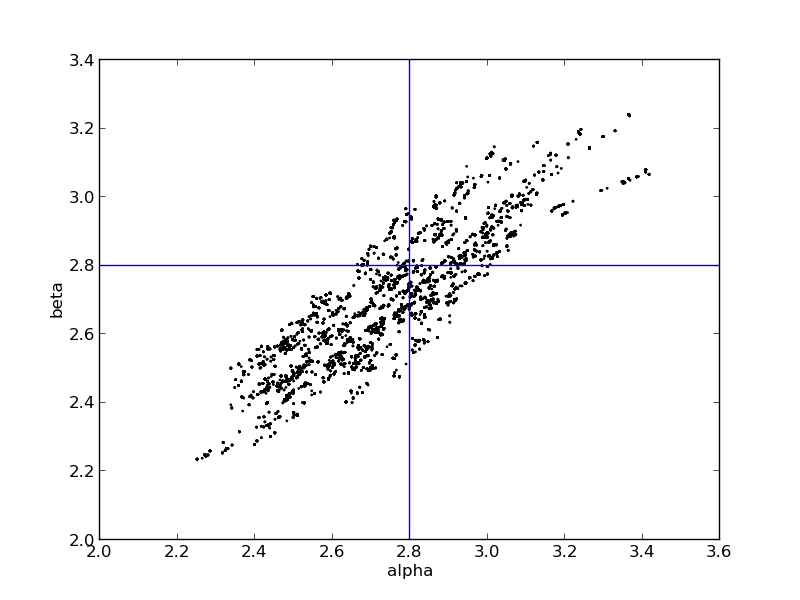
\includegraphics[scale=0.5]{uni/alpha_beta}

Since the value of |g| is usually supposed to be less than 0.1. While
comparing with traditional average method,in this paper the distribution
of ``true'' g is a uniform distribution within -0.1\textasciitilde{}0.1
for both g1 and g2.

To compare the accuracy with traditional averaging method we calculate
the value of $\sqrt{mean(\hat{g}}-g^{true})^{2}$

for HB method the typical value is \textasciitilde{}0.17 While for
traditional averaging method it's \textasciitilde{}0.18.

Though the value of mean square error depends on specific mock data
used,HB method consistantly out perform traditional averaging method
on a level of \textasciitilde{}0.01


\subsubsection{Step function model}

In this section we do not suppose the intrinsic distribution of ellipticity
to be Beta distribution any more.Instead we use a histogram to describe
the dtistribution of intrinsic ellipticity.We divide the 2-D space
r$\in$(0,1) into 10 bins .The probability of each bin is $p_{i}=e^{\alpha_{i}}$
.$\overrightarrow{\alpha}$ is a 10D parameter vector to be infered.

From practice we find that a prior smooth regularzation on $\alpha$
is needed to obtain a good estimation on shear g.

The prior distribution we used on $\alpha$ is : 
\begin{equation}
Prior(\alpha)=exp(-\xi*\sum(\alpha_{i}-\alpha_{i-1})^{2})
\end{equation}


As in the Beta function model section,the data we used is 64{*}8 galaxies
seperated in 64 sky patches,and the prior of g is also the same.

$\xi$ is fixed at 2 .

Inital state is still the result of traditional average .

.Figure 8 shows the samples of g for 64 patches and 8 galaxies in
each patch and Figure 9 shows the infered $\vec{\alpha}$.The red
line in Figure 9 is Beta(2..8,2.8) the distribution used in data generation
part.

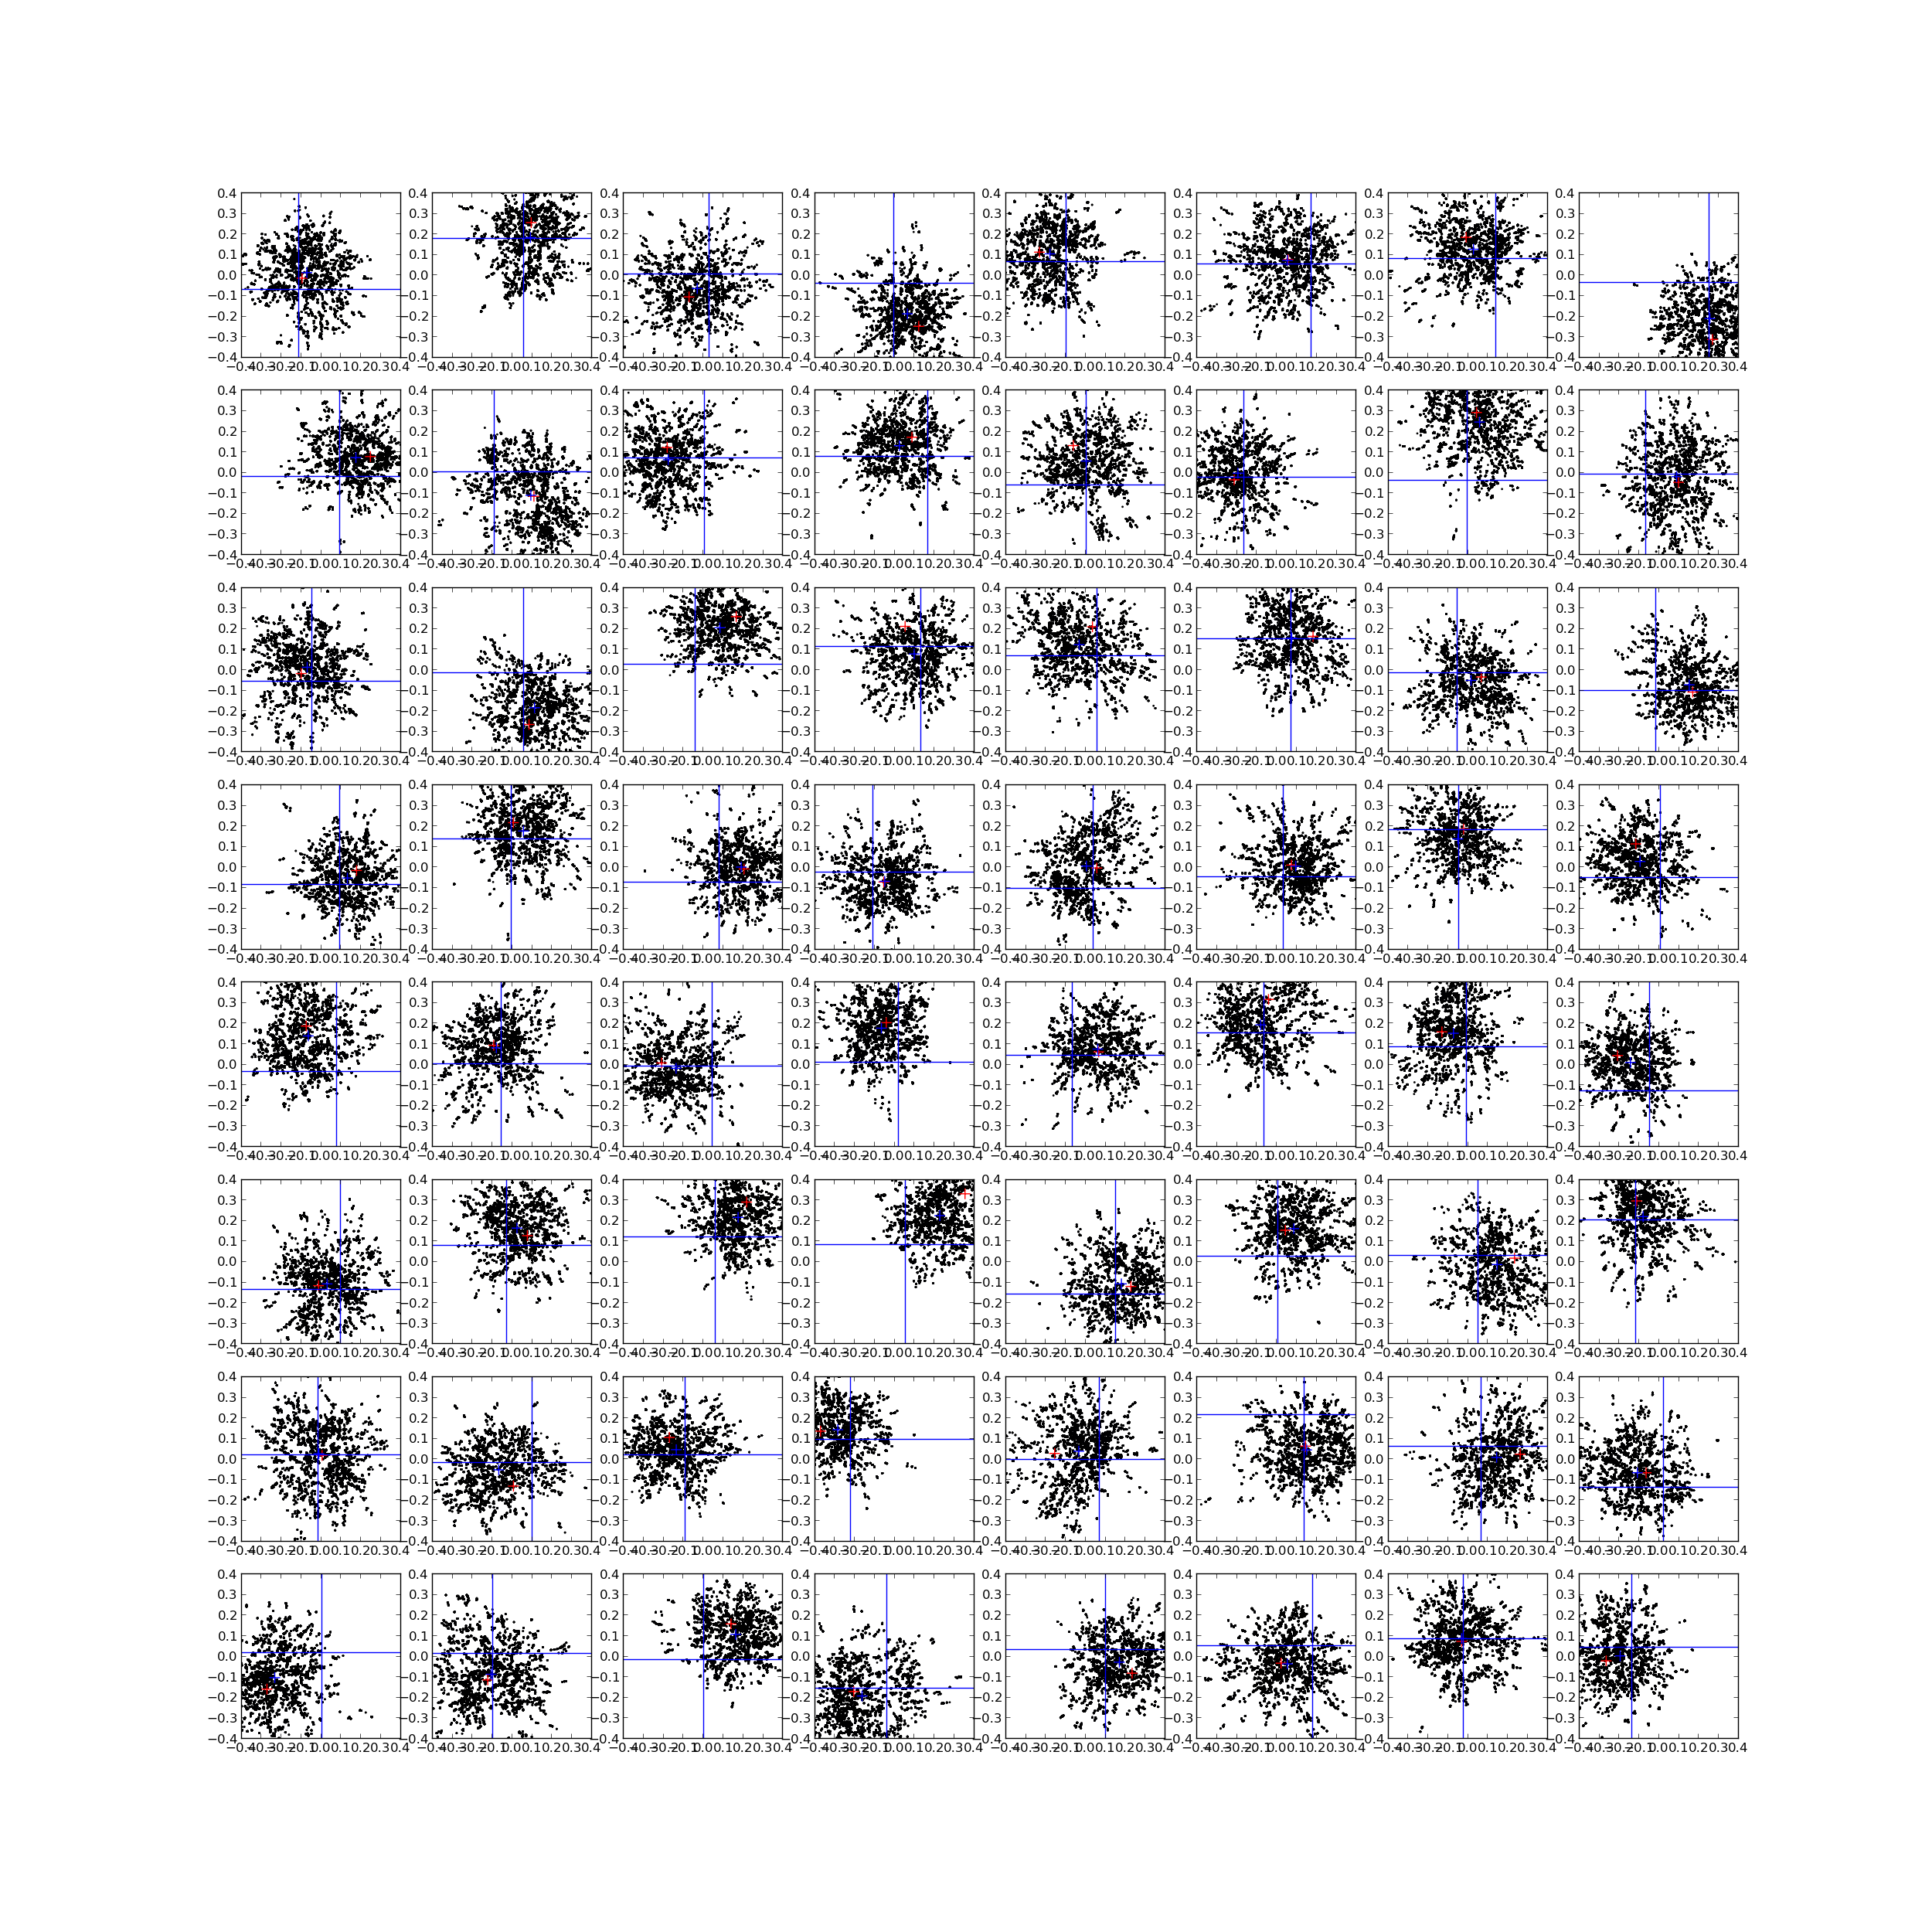
\includegraphics[scale=0.2]{step/test10}Figure 8

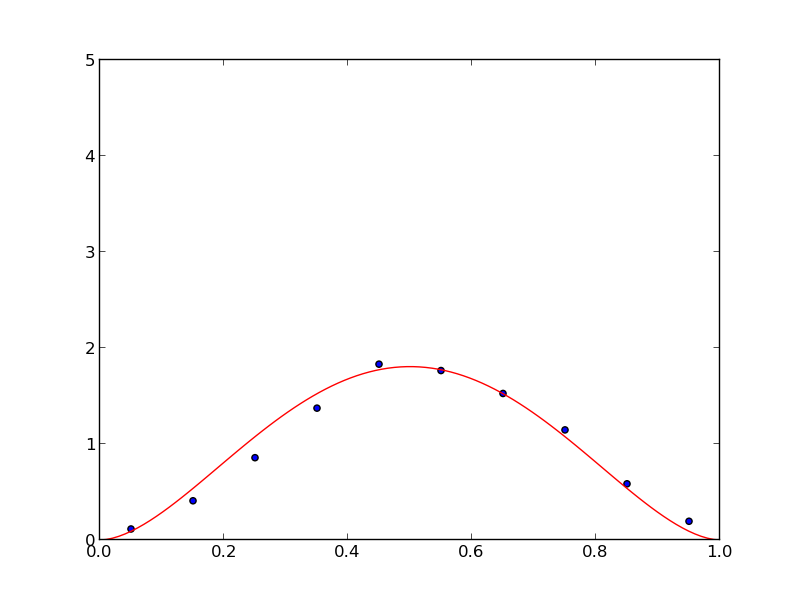
\includegraphics[scale=0.5]{step/stp10}

figure 9.The blue points are the infered $\alpha$ at the bin centers.Red
linr is true distribution Beta(2.8,2.8)

The accuracy we got from beta function model and step function model
are similar.They both out perform the traditional average method by
percentage level.

Figure 10 shows how the mean square error of the Hierarchy Bayesian
method varies with the number of sky patches used,in comparison with
traditional average method and likelihood analysis with correct P($\epsilon$)
hard-set.from this figure we can see that the mean square error of
the Hierarchy Bayesian method decreases as the number of patches goes
up,while this trend is less significant as number of patches becomes
larger.Moreover,down to 8 patches this Hierarchy Bayesian method still
out perform the traditional average method. Meanwhile the likelihood
analysis with correct P($\epsilon$) shows higher accuracy than Hierarchy
Bayesian method. That is consistent with our speculation. When the
number of patches goes to infinity ,we will have correct estimation
on P($\epsilon$) and Hierarchy Bayesian method converges to likelihood
analysis with correct $P(\epsilon)$ hard-set,ignoring the difference
between our step function model and real beta function,of course.

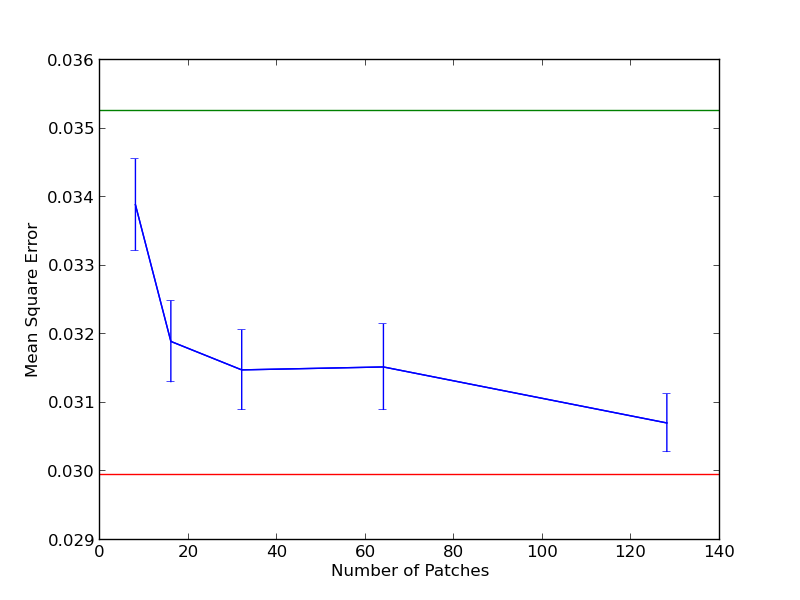
\includegraphics[scale=0.5]{Np_step}

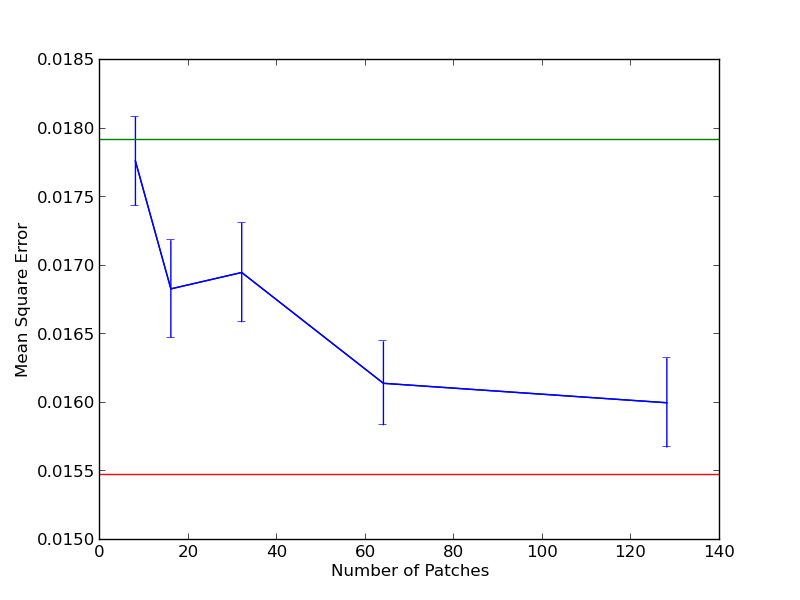
\includegraphics[scale=0.5]{N16NP_vary}

Figure 10:Mean square error VS Number of patches.In the upper graph
number of galaxies per patch is 8 while in the lowwer it's 16.The
Green line is mean square error of traditional average while the red
line is that of likelihood analysis with correct $P(\epsilon)$ .


\subsection{Shape Measurement Error}

In this part we will discuss how the shape measurement error will
affect the relative accuracy of this Hierarchy Bayesian method.As
mentioned before ,we try to avoid any image process which is another
important aspect of Weak Lensing survey ,so we simply assume a 2D
Gaussian noise on ellipticity measurement.

With that Gaussian noise the data we can obtain becomes the observed
ellipticity $\epsilon_{ob}$,whoes probability distribution is 
\begin{equation}
f(\epsilon_{ob}|\epsilon_{\ell})\varpropto e^{-\frac{(\epsilon_{ob}-\epsilon_{\ell})^{2}}{2\sigma^{2}}}
\end{equation}


Therefore the likelihood of $g$ and $\alpha$ becomes
\begin{equation}
L(g,\alpha|\epsilon_{ob})=P(\epsilon_{ob}|g,\alpha)=\intop f(\epsilon_{ob}|\epsilon_{\ell})P(\epsilon_{\ell}|g,\alpha)d\epsilon_{\ell}
\end{equation}



\section{Systematic Bias}

In this section,we measured the levels of possible systemmatic bias
led by this HB method.

Following Heymans et al. (2006), we quantify the systematic bias in
in terms of the multiplicative error m and additive error c on the
true shear $g^{true}$ 
\begin{equation}
\hat{g_{i}}-g_{i}^{true}=m_{i}g_{i}^{true}+c_{i}
\end{equation}


The accuracy in Weak Lensing measurement depends on both galaxies
shape measurement and shear inference period.In this paper our main
concern is how to infere shear in a HB method instead off traditional
averaging method and it does not involve the shape measurement part
.Therefore we assume we have perfect galaxies ellipticity measurement,and
all the possible inaccuracy is due to this HB shear inference method.

Using 10,000 data sets we are able to get the value of m and c for
both beta function and step function model.Each data set we use in
this section has 64 patches with 8 galaxies in eah patch.

The region for $g_{i}^{true}$ is -0.1\textasciitilde{}0.1 .

For beta function model :

\begin{tabular}{|c|c|c|}
\hline 
 & Expect Value  & STD\tabularnewline
\hline 
\hline 
m1  & -0.00420  & 0.00304\tabularnewline
\hline 
c1  & 1.66$*10^{-4}$  & 1.73$*10^{-4}$\tabularnewline
\hline 
m2  & -0.00386  & 0.00290\tabularnewline
\hline 
c2  & 2.30$*10^{-4}$  & 1.81$*10^{-4}$\tabularnewline
\hline 
\end{tabular}

For step function model:

\begin{tabular}{|c|c|c|}
\hline 
 & Expect Value  & STD\tabularnewline
\hline 
\hline 
m1  & 0.00502  & 0.00287\tabularnewline
\hline 
c1  & 2.05$*10^{-4}$  & 1.73$*10^{-4}$\tabularnewline
\hline 
m2  & 0.00156  & 0.00292\tabularnewline
\hline 
c2  & 2.14$*10^{-4}$  & 1.87{*}$10^{-4}$\tabularnewline
\hline 
\end{tabular}

\includegraphics[scale=0.5]{step_g1}

\includegraphics[scale=0.5]{g2_step} 
\begin{quote}
Figure 9: Linear fit of $\delta g_{i}-g_{i}$ relationship for step
function model. 
\end{quote}
As we can see from the data and graph no significant systematic bias
can be found using 10,000 data sets.With that amount of data we able
to narrow down m to $\sim10^{-3}$ and c to $\sim10^{-4}$.

In Table 1 we show the requirements on m, c for current, upcoming
and future cosmic shear surveys (Joe Zuntz ,axrive 2013)

\begin{tabular}{|c|c|c|}
\hline 
 & m  & c\tabularnewline
\hline 
\hline 
current  & 0.02  & 0.001\tabularnewline
\hline 
upcoming  & 0.004  & 0.0006\tabularnewline
\hline 
future  & 0.001  & 0.0003\tabularnewline
\hline 
\end{tabular}

Compare this table with our data,we can see that our method can at
least support upcoming cosmic shear surveys.Note that we only used
10,000 data sets to quantify m,c due to limited computing time and
the uncertainty on $\hat{g}$ is large(\textasciitilde{}0.1),if much
more data sets were collected, these number will probably be significantly
lowered.


\section{Conclusion}

Here we present a Hierarchy Bayesian method of shear inference. Our
method successfully infers the cosmic shears of different sky patches
and the intrinsic shape parameter synchronously.We showed that in
the area that galaxy density is low,our method can out perform traditional
averagemethod by \textasciitilde{}0.01 level. While in most cases
cosmic shear is just around this level. Also we quantify the level
of multiplicative and additive error,and shows this method has no
sign of a systematic bias down to (m\textasciitilde{}$10^{-3}$ c\textasciitilde{}$10^{-4}$
level ) and that this method can be aiming at support upcoming shear
surveys.

Eventhough the number of parameters used in this paper is up to 138
,using Gibbs sampler and starting from the result of simple average
we are able to make MCMC chain converged within 25s.

Further more ,by using the step function model, we showed that this
Hierarchy Bayesian method does not require correct knowledge on the
model of intrinsic shape dstribution.Simply using a step function
model and a prior regulazier we were able to get similar result as
when we assume we know the correct model of intrinsic shape distribution.

One intresting in shear survey is that the assumption that galaxy
pairs have no ellipticity correlation is not entirely accurate. There
are intrinsic alignments of nearby galaxies due to the alignment of
angular momentum produced by tidal shear correlations( Heymans C.,
Brown M., Heavens A., Meisenheimer K., Taylor A., Wolf C., 2004, MNRAS,
347, 895 ;B. Casaponsa, A. F. Heavens, T. D. Kitching, arxive,2013).Consider
the ellipticity the first assumption of traditional average method
$<\epsilon_{0}>=0$ does not stands any more,while for this Hierarchy
Bayesian method though we are also using the assumption that intrinsic
orientational angle distribution is a flat distribution, we can just
re-model it once more information on galaxy shape coorelation is uncovered. 
\end{document}
